% Appendix: proof sketch, statistical procedures, index of corrections, supporting figures.
% Order here is the printed appendix order; each part keeps its own \section and \label.

\section{Proof sketch for Proposition~\ref{prop:ident}}
\label{app:proof}
Let atom $a$ have Cartesian position $p \in \mathbb{R}^3$ and let $v, w$ be two views with linearly
independent directions $d_v, d_w$. Its images are $q = P_v p$ and $q' = P_w p$. The back-projections are
the affine lines $\ell_v = \{x : P_v x = q\}$ (direction $d_v$) and $\ell_w = \{x : P_w x = q'\}$
(direction $d_w$). Both contain $p$; since $d_v \not\parallel d_w$, two non-parallel lines in
$\mathbb{R}^3$ that intersect do so in exactly one point, so $\ell_v \cap \ell_w = \{p\}$ and the
intersection step of Algorithm~\ref{alg:oracle} recovers $p$ exactly from the correct pairing. It remains
to show no incorrect pairing survives. A spurious pairing $(q, q'')$ with $q''$ the image of a different
atom $b$ either yields no intersection (skew lines, rejected) or yields a point $\hat{p} \neq p$ whose
projections must, by hypothesis (ii), fall outside the matching tolerance of any same-species point in at
least one remaining view, so the verification step rejects it. The verified reconstruction is
therefore exactly the atom set, on which $\spg$ returns $y(s)$ by the definition of the label. Condition (ii) is where the argument is not vacuous: it fails precisely on projective coincidence, when
distinct atoms project within tolerance of one another in the verifying views. The measured ceiling gap
(0.0476 on the original sample) and its growth with atoms per cell (Section~\ref{sec:controls}) are
measurements of that failure set.


\section{Statistical procedures}
\label{app:stats}
\textbf{Paired comparisons.} Every model-versus-model and model-versus-oracle comparison on a shared sample
is a paired exact binomial (sign) test on discordant structures: with $g$ structures one arm alone gets
right and $l$ the other alone, the two-sided $p$ is that of $\mathrm{Bin}(g+l, 1/2)$ evaluated at
$\min(g,l)$. For the render-convention probe, the per-comparison minimum detectable difference is the
smallest $|g-l|/n$ reaching $p<0.05$ given that comparison's observed $g+l$; with $g+l \le 5$ no split
reaches it, which is the source of the 7-of-16 unreachable comparisons in
Section~\ref{sec:conventions}.
\textbf{Label certification.} The one-sided exact 95\% lower bound for $k/k$ agreements is
$0.05^{1/k}$; for $k = 220$ this is $0.9865$.
\textbf{Run-to-run spread.} The second sweep execution is retained as a labelled replication; spread is
reported as the mean and maximum absolute per-model difference in correct counts.


\section{Index of corrections and non-recoveries}
\label{app:corrections}
The full retraction ledger, verbatim and in checkpoint order, is in the supplementary. Main-text items:
the retired below-baseline claim (Section~\ref{sec:controls}), the retracted unpaired
minimum-detectable-difference (Section~\ref{sec:conventions}), the withdrawn stratified-accuracy mechanism
(Section~\ref{sec:controls}), and the three documented non-recoveries (Limitations).


\section{Supporting figures}
\label{app:secondary}
The visibility-conditioned oracle of Section~\ref{sec:conventions} and the two secondary axes of
Section~\ref{sec:controls} are stated numerically in the main text; their figures are placed here.

\begin{figure}[htbp]
\centering
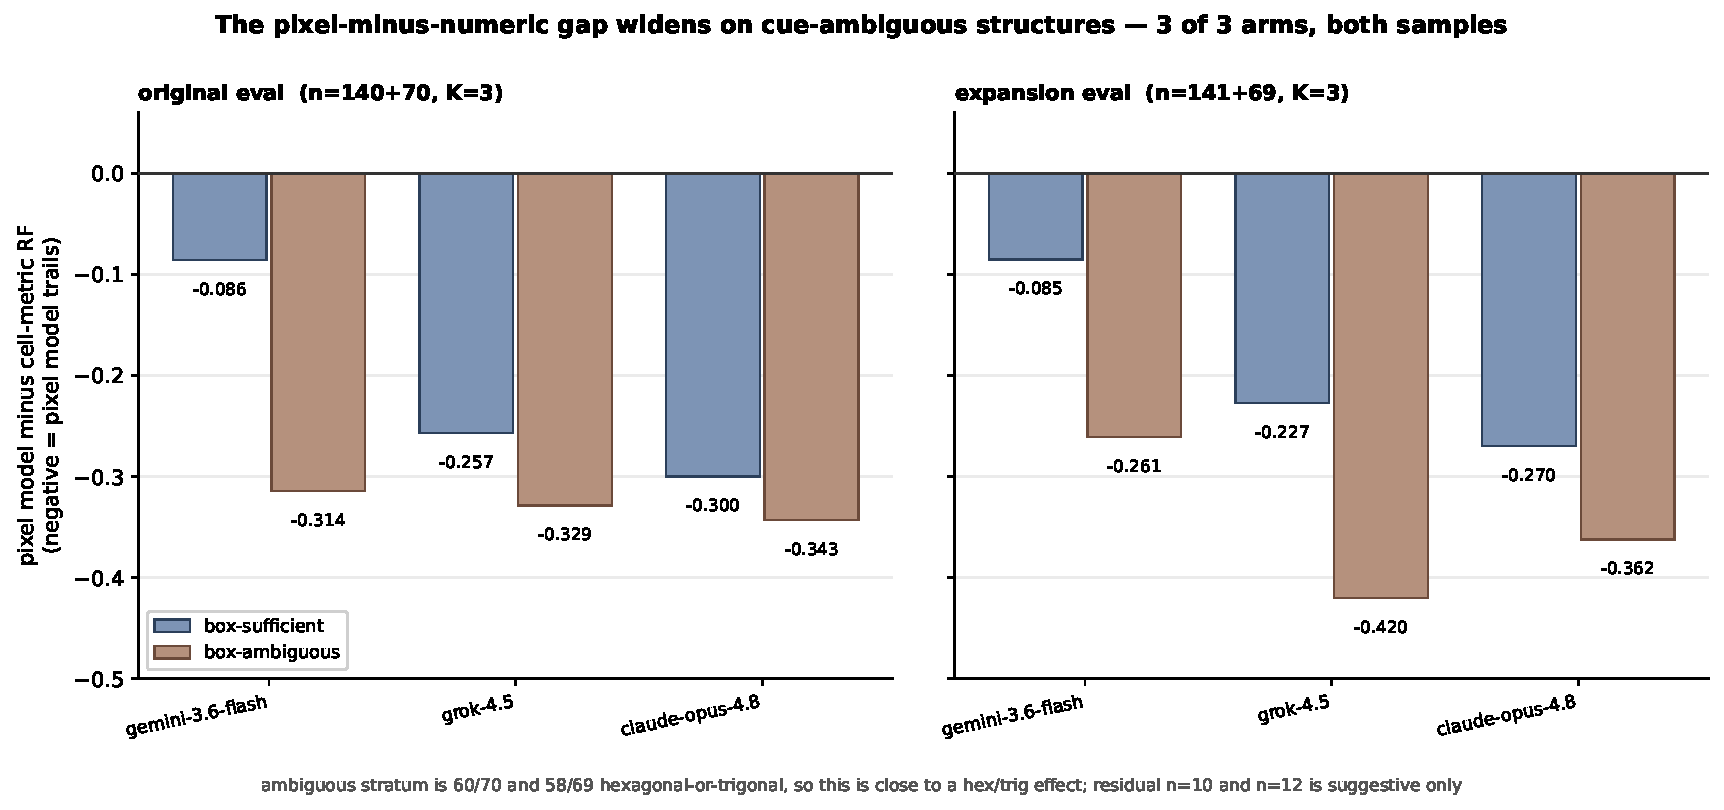
\includegraphics[width=0.8\linewidth]{figures/cuesuff.pdf}
\caption{Pixel accuracy minus a cell-metric random forest on the same structures, by cue-sufficiency
stratum, three frontier models, both evaluation samples ($K=3$). Negative means the pixel model trails the
numeric reader. Stratum composition is annotated on the panels; see Section~\ref{sec:controls}.}
\label{fig:cuesuff}
\end{figure}

\begin{figure}[htbp]
\centering
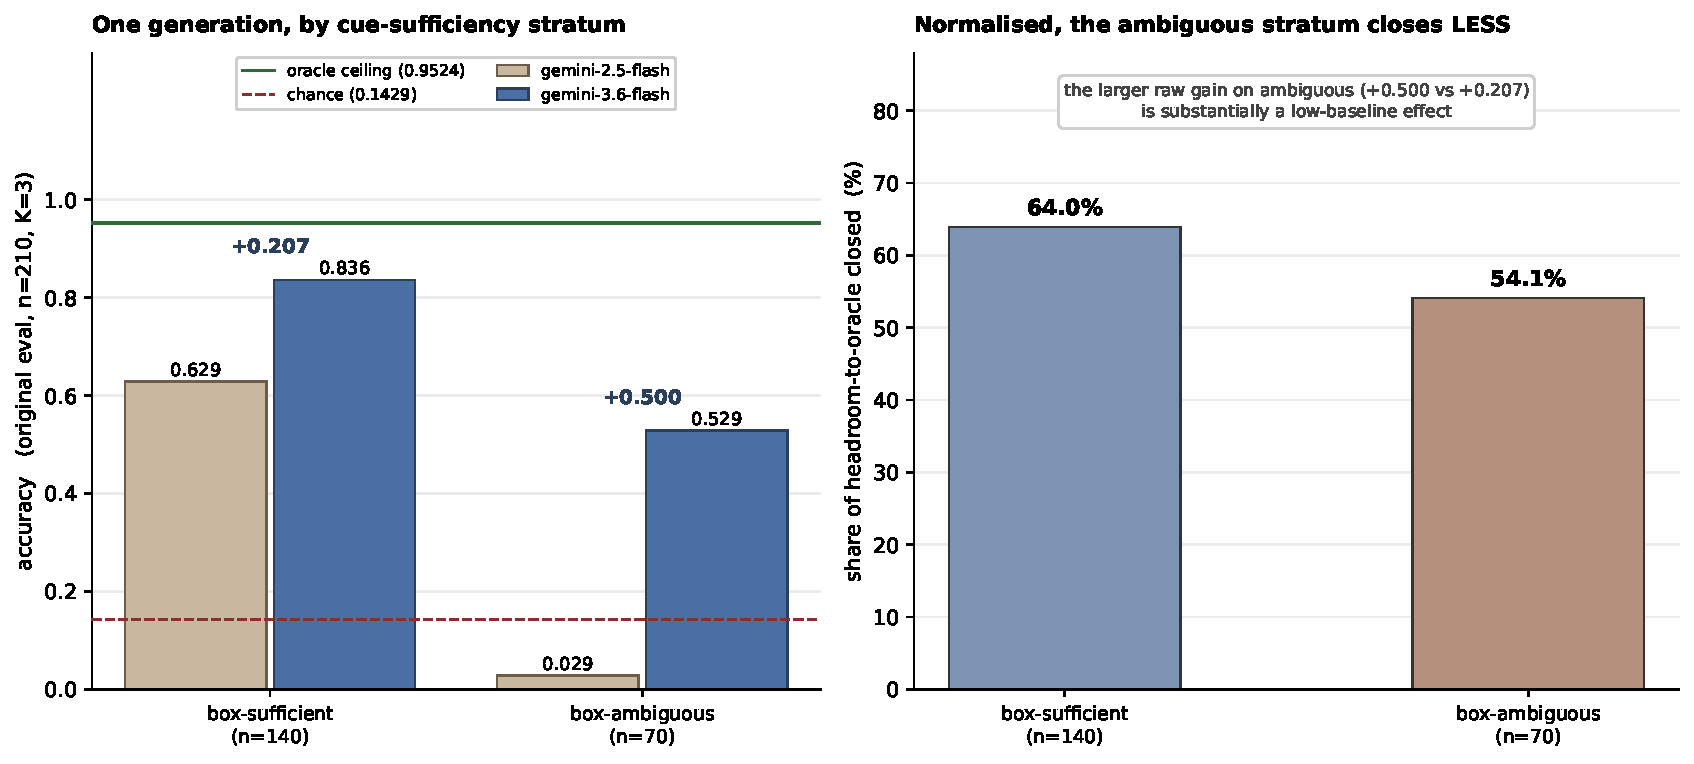
\includegraphics[width=0.8\linewidth]{figures/generational.pdf}
\caption{One generation of model progress, original sample, $n=210$, $K=3$. Left: raw accuracy by
cue-sufficiency stratum, with the oracle ceiling and seven-way chance drawn. Right: the same gains
normalised by headroom to the oracle.}
\label{fig:generational}
\end{figure}

\begin{figure}[htbp]
\centering
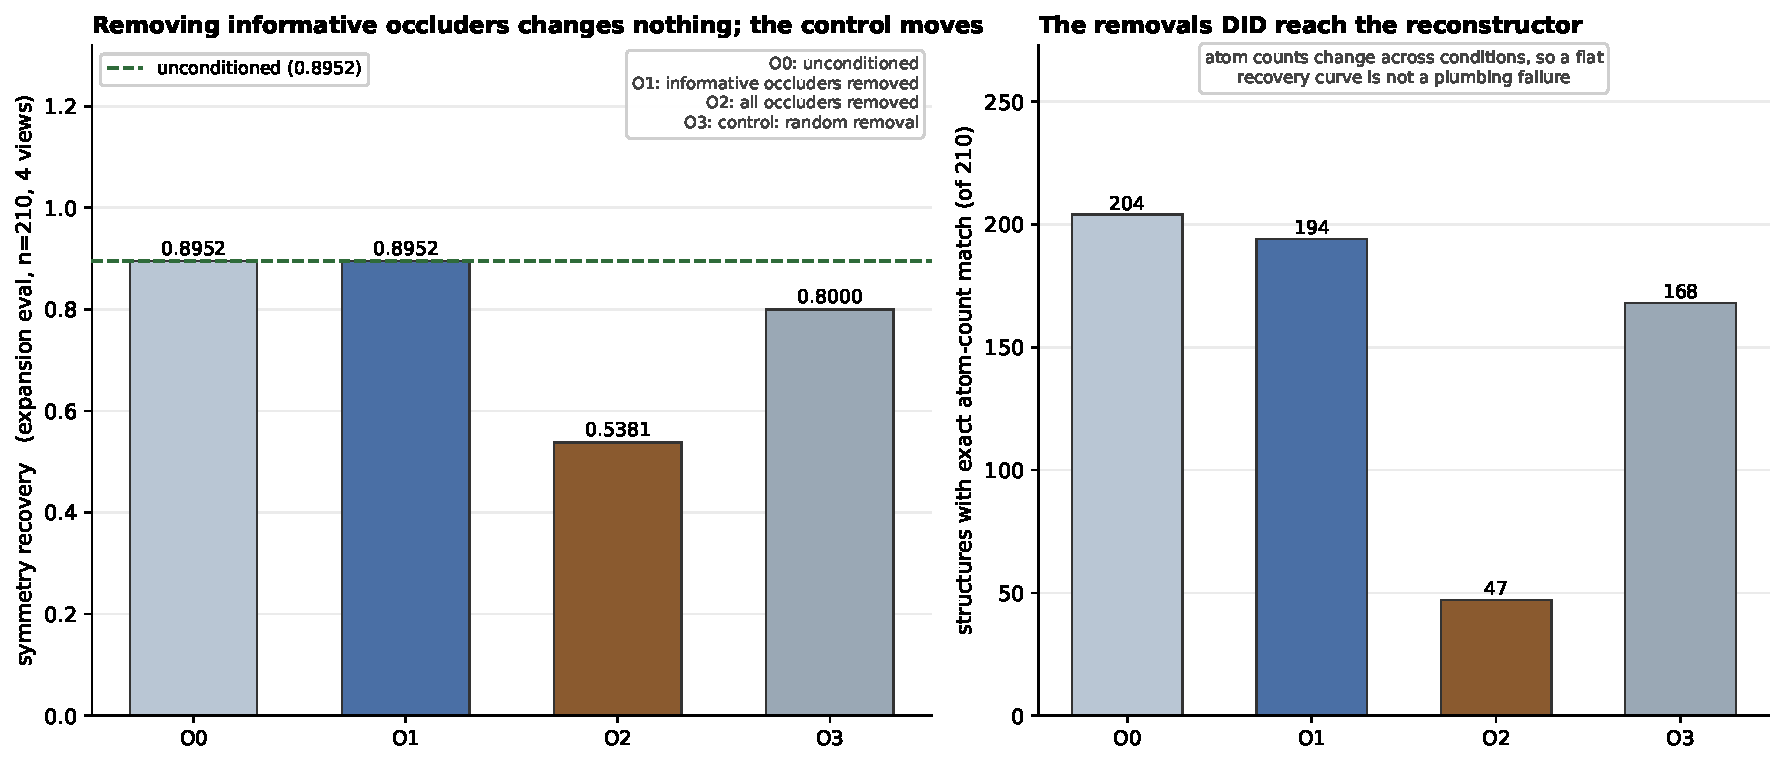
\includegraphics[width=0.8\linewidth]{figures/conditions.pdf}
\caption{Visibility-conditioned oracle: recovery when informative occlusion is removed from the oracle's
input, when redundant occlusion only is removed (pre-registered control), and unconditioned, on both
evaluation samples.}
\label{fig:conditions}
\end{figure}
